%!TEX root = Report.tex
\chapter{Measurements And Results}\label{sec:results}

\section{Calibration process}
As mentioned above the TLC had to be calibrated. This is quiet a time-consuming procedure, because the assumptions is made that the temperature change proceeds quasi-stationary implying that after each step thermal equilibrium is reached. RGB-data from the camera is converted to HSI and after polynomial interpolation the Hue-value correlates with the temperature as shown in figure \ref{fig:calibration}.

\begin{figure}[H]
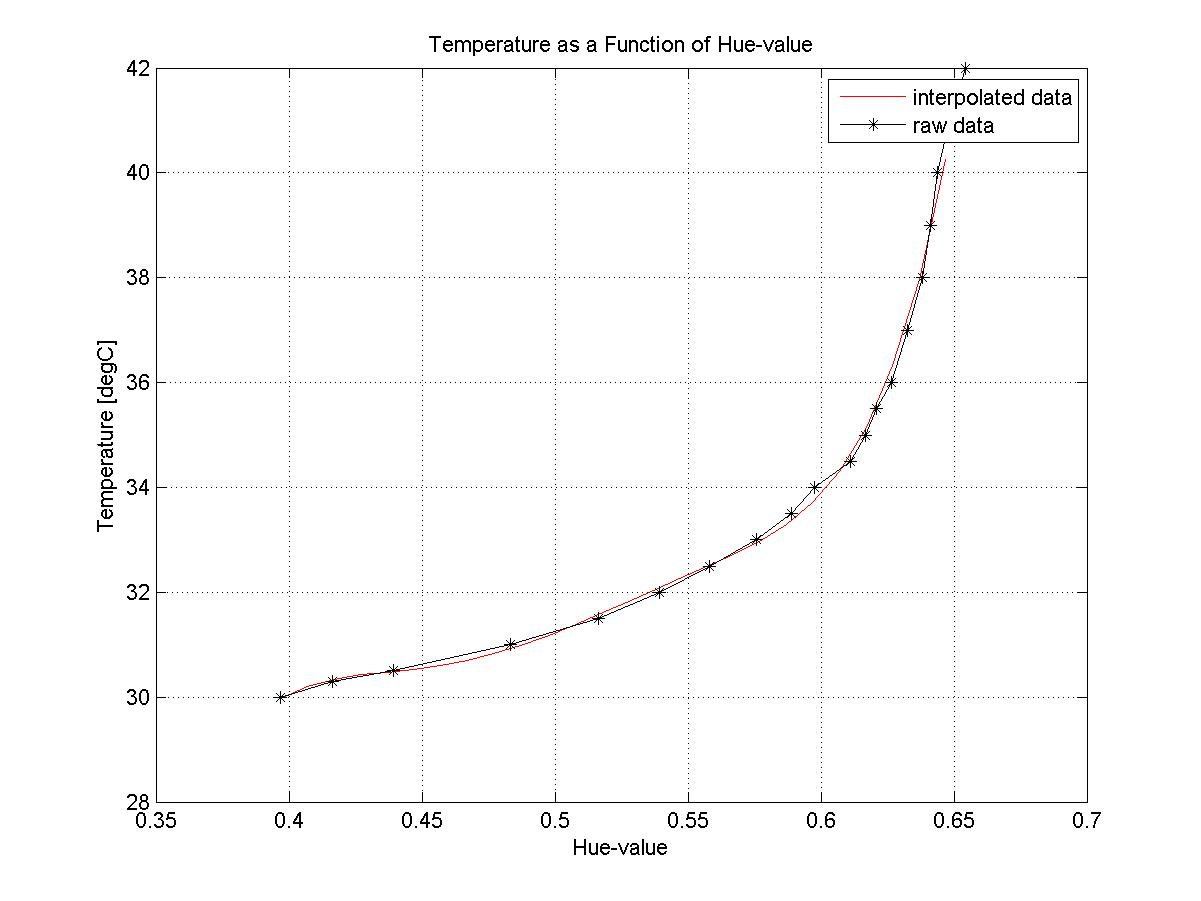
\includegraphics[width=0.95\textwidth]{pics/calibration}
\caption{Temperature as Function of Hue Value}
\label{fig:calibration}
\end{figure}


\section{Measurements}
The measurements we took did not yield to any meaningful result, because the camera didn't record the propagating front of cold water and thus no change in color was observed.
\section{Qualitatively Correct Results}
However the advisor provided us with reasonable results from a previous run of the experiment shown in figure \ref{fig:temperature} below. The camera took 100 pictures but only frame 1 to 12 depict a change in color. It seems like the cold water pulse already passed the test section and only the last part of the temperature drop is represented.
\begin{figure}[H]
\centering$
\begin{array}{cccccc}
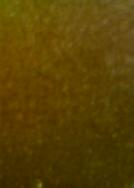
\includegraphics[width=.14\textwidth]{pics/91} &

\includegraphics[width=.14\textwidth]{pics/92} &

\includegraphics[width=.14\textwidth]{pics/93} &
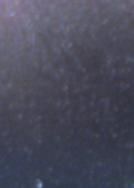
\includegraphics[width=.14\textwidth]{pics/94} &

\includegraphics[width=.14\textwidth]{pics/95} &

\includegraphics[width=.14\textwidth]{pics/96} \\
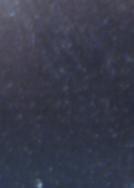
\includegraphics[width=.14\textwidth]{pics/97} &

\includegraphics[width=.14\textwidth]{pics/98} &
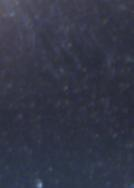
\includegraphics[width=.14\textwidth]{pics/99} &

\includegraphics[width=.14\textwidth]{pics/910} &
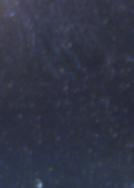
\includegraphics[width=.14\textwidth]{pics/911} &
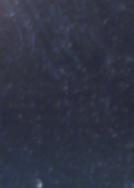
\includegraphics[width=.14\textwidth]{pics/912} 
\end{array}$
\caption{Change of Color Picture 1 to 12}
\label{fig:temperature}
\end{figure}


Eventually the MATLAB script computed the heat transfer coefficient $\alpha$ and the surface temperature $T_s$ and plotted the values in function of time displayed in figure \ref{fig:alpha} and figure \ref{fig:surfaceT}. Apparently initial conditions for the computation are defined wrong yielding to very high values of $\alpha$ and very low temperatures at the beginning of the experiment. Between $t=0.4\ s$ and $t=2\ s$ an exponential temperature decline is observed. Furthermore the heat coefficient goes up and down although it should be constant yielding in a rough average of $\alpha = 8\ kW/m^2K$.

\begin{figure}[H]
\mbox{
\subfigure[]{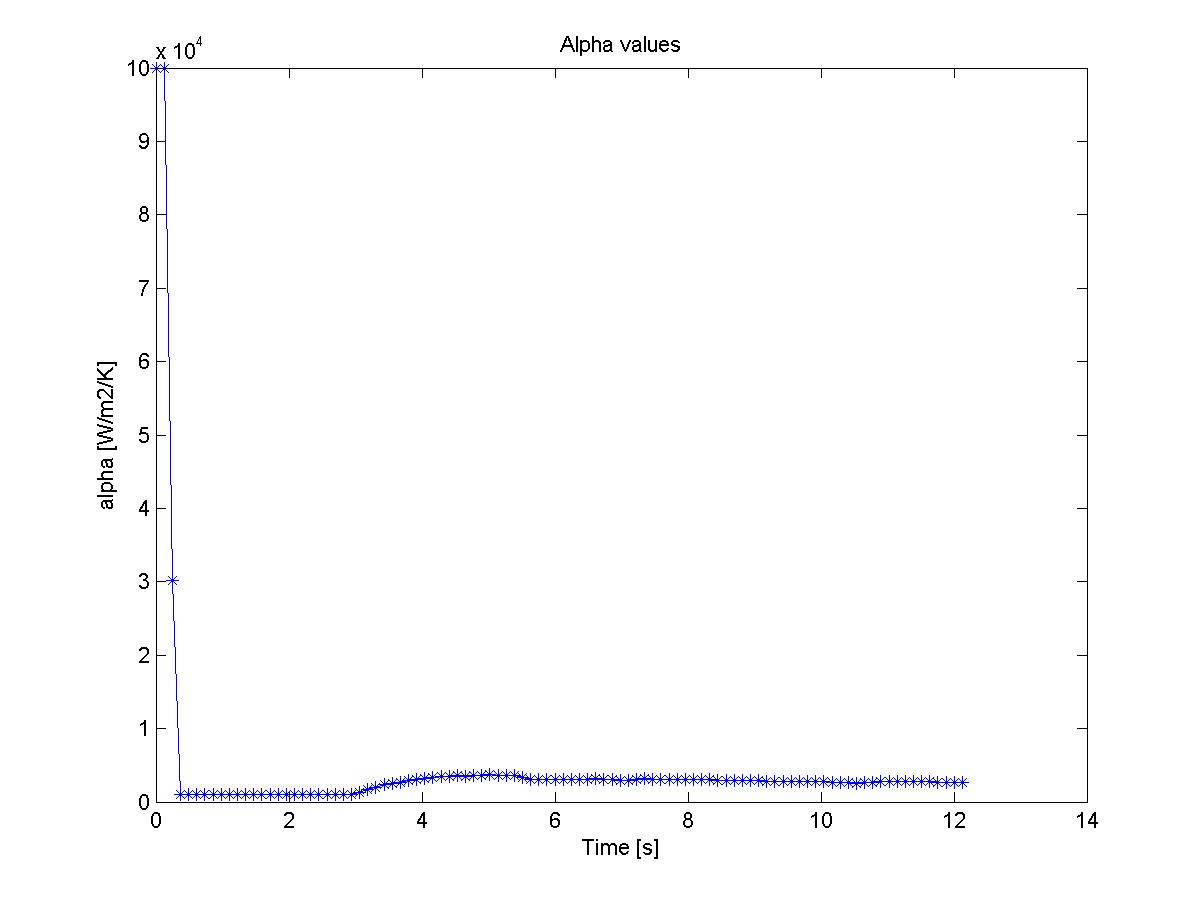
\includegraphics[width=.5\textwidth]{pics/alpha}
\label{fig:alpha}}\quad
\subfigure[]{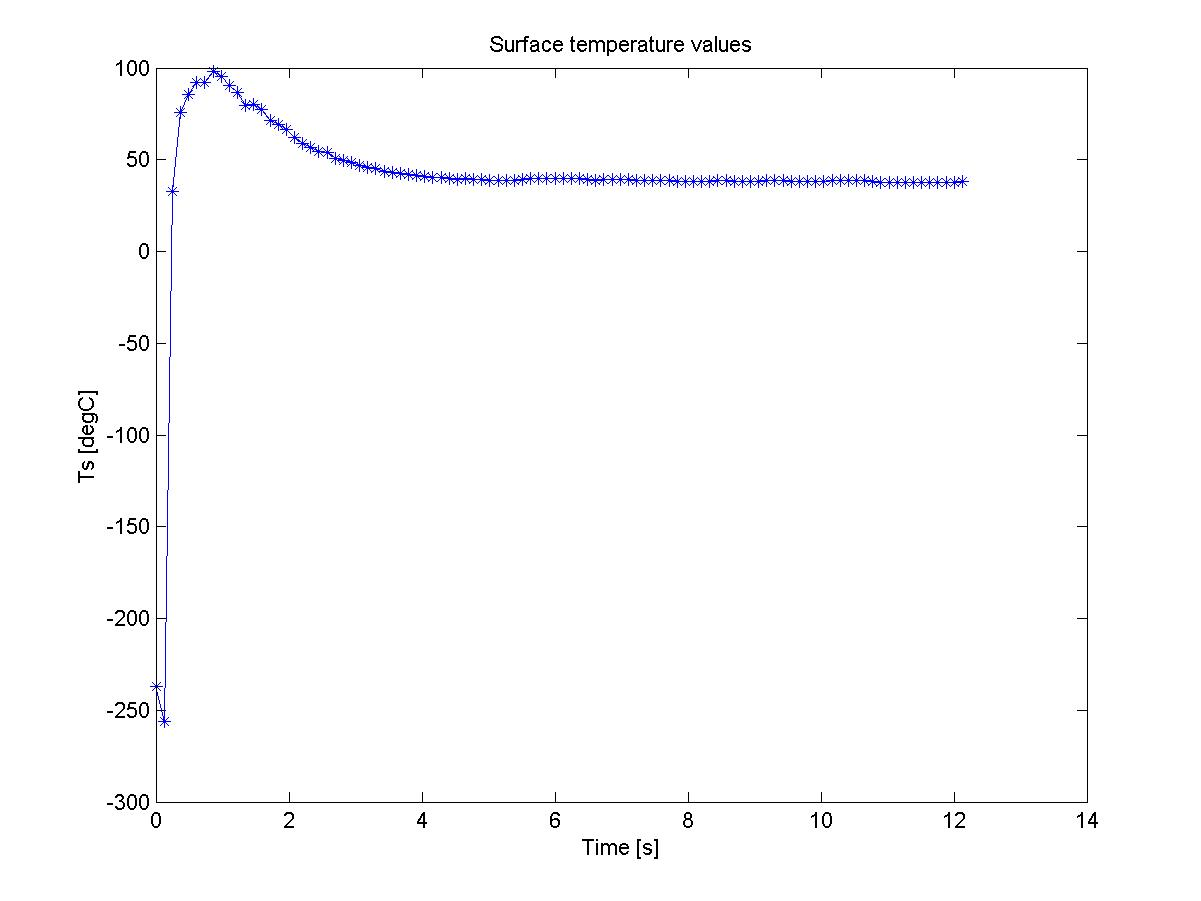
\includegraphics[width=.5\textwidth]{pics/surfaceT}
\label{fig:surfaceT}}}
\caption{(a) Heat Transfer Coefficient (b) Surface Temperature over Time}
\label{pic:surfaceT}
\end{figure}
